\documentclass{article}
\setlength{\parindent}{0pt}
\usepackage{graphicx} % Required for inserting images
\usepackage{minted}
\usepackage{float}  % 加载float包


\title{Background Chapter}
\author{Yu Jason}
\date{October 2024}


\usepackage{listings}
\usepackage{xcolor}

\lstset{
    language=C++,                % 设置代码语言
    basicstyle=\ttfamily,        % 基本字体样式
    keywordstyle=\color{blue},   % 关键字颜色
    stringstyle=\color{red},     % 字符串颜色
    commentstyle=\color{green},  % 注释颜色
    numbers=left,                % 显示行号
    numberstyle=\tiny\color{gray}, % 行号的样式
    stepnumber=1,                % 每行显示行号
    breaklines=true,             % 自动换行
    tabsize=4              % Tab 宽度
}


\begin{document}

\maketitle

\section{Background Chapter}
Libseff is a library that designed to provide an effect handler functionality directly to a C programmer. Effect handler is a mechanism that used to handle side effects in a program. These side effects happens when a program that interact with the external environment or change state during computation, e.g., I/O, exception handling, concurrency, state changes, etc. However, there already has two C effect handler libraries, libhandler[1] and libmpeff[2]. The key difference is, they are mainly designed for compiler developers and use as compilation targets for high-level programming languages rather than as tools for C programmers to use directly. In other words, these two libraries are more suitable for use in compiler generated code, not for C programmers to use directly or to call. And the difference between traditional effect handler implmentation is libseff use mutable coroutine object rather than immutable continuation object this means when executing effect operation we don't need to allocate new continuation object every time. Since there is no need to frequent create a new continuation object means that the cost of allocate memory is reduced, this improves the performance and reduced the memory usage[3].
\medskip

The figure 1 shows a simple implementation of using effect handlers.

\begin{figure}[H]
    \centering
    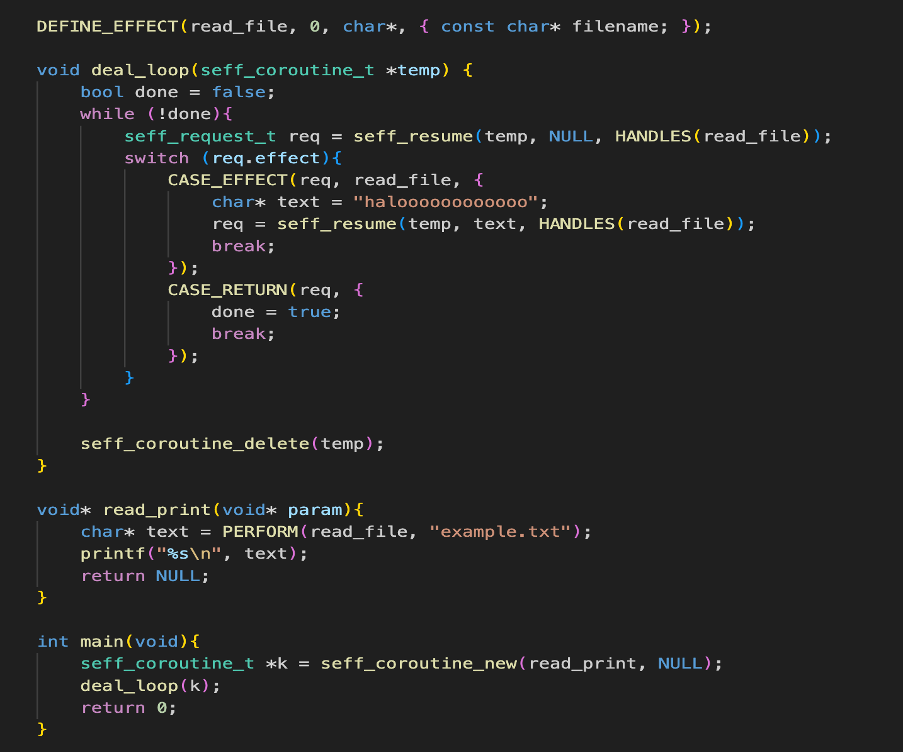
\includegraphics[width=0.7\textwidth]{image.png}
    \caption{Enter Caption}
    \label{fig:enter-label}
\end{figure}

\begin{lstlisting}
DEFINE_EFFECT (read_file, 0, char*, {const char* filename; });
\end{lstlisting}

Here we define an effect called \texttt{read\_file}, it has tag 0 and takes \texttt{const char*} as a parameter type, which in this case is a filename. The return type is \texttt{char*}, representing the content of the file. This defines the form and interface of the \texttt{read\_file} effect.

\begin{lstlisting}
void deal_loop (seff_coroutine_t *temp)
\end{lstlisting}

Here we use \texttt{deal\_loop} to handle the effects based on the requests made by the coroutine. The \texttt{seff\_resume} function is used to resume the coroutine, where \texttt{temp} is the coroutine object. The effect that the coroutine has requested is contained in the \texttt{seff\_request\_t} object returned by the \texttt{seff\_resume} function. We use a \texttt{CASE\_EFFECT} branch to handle the \texttt{read\_file} effect once it is identified. In this case, we simulate the read file operation, not actually read the file. Then, the coroutine is resumed with the text "haloooooooooooo" passed as the result to the coroutine, and the loop will exit when the \texttt{CASE\_RETURN} branch has handled the coroutine's completion.

\begin{lstlisting}
void* read_print (void* param)
\end{lstlisting}

We create a coroutine function called \texttt{read\_print}. What it does is try to perform the \texttt{read\_file} effect, which is to request a file operation to read the content from "example.text" and print it, then return.

\begin{lstlisting}
int main(void)
\end{lstlisting}

This main function first creates a new coroutine called \texttt{k}, passing in the \texttt{read\_print} function, and then lets \texttt{deal\_loop} handle all the effect requests from this coroutine until it completes.

\medskip




This simple demonstration shows how to use an effect handler to handle effects in the coroutine. A coroutine can stop itself and request an effect through the effect handler (e.g., \texttt{read\_file}), and then handle it outside, like in \texttt{deal\_loop}, which will give the result and resume the execution of the coroutine. This design is similar to an asynchronous mechanism, completing asynchronous tasks without blocking the main program.

\medskip
\medskip

Stack management is one of the most important concept in libseff  library, to be more specific we need to decide how to allocated stack frame and resized it. Stack frames are the memory space used by function calls at program runtime, and how these stack frames are managed in a coroutine implementation is a key issue. In a other word different stack management strategies can result in different performance and memory usage of the program. In libseff library there already exists two stack management strategies which is Fixed-Size Stacks and Segmented Stacks which can be selected individually.

\medskip

Fixed-Size Stacks is the most simple method to manage a stack as it don't have to resize the stack dynamically, the only thing it has to do is allocate a fixed size block of the memory for coroutine when it has been created. The advantage of this approach is it's easy to implement also there is no additional runtime cost as the size of the stack is fixed and there is no need to adjust the memory during the operation. but there is a trad-off, we have mentioned that the size of the stack is fixed so that could cause memory wasted if the actual needed memory is less than the allocated memory that means the part of the unused memory will be wasted. and is hard to predict the exact memory needed if allocated memory is too small it could cause a stack overflow, if it was overly allocated that will waste large amount of memory, but to avoid the stack overflow, we normally give out memory way more than it's actual need to avoid the stack overflow increase the risk of memory wastage.

\medskip

Segmented stack is designed to achieve first-class continuation more efficiently and it has a call stack structure[4]. Continuation is a concept in programming, that represent the next step of the current computation work, the program can capture the current execution status and resume execution in any point by using continuation. First-class means this concept can be just like a normal variable that can be passed, stored and manipulated. 

\medskip


The concept of the segmented stack is change fixed size stack to linked multi stack segment or "stackelets" to manage the stack, and each function will check if the current stack has enough space for the new stack frame at runtime, if not, the system will allocate a new stack segment means that it has dynamic stack size, which reduce the risk of stack overflow and improve flexibility by using morestack function. although there are many advantage of using segmented stack but there are some previously unknown problems which may be the one of the reason why it have poor memory efficiency and performance in the past, there also has a well-known problem for the segmented stack known as "hot-split"[6,7,8]

\medskip

"hot-split" is a kown problem related to segmented stack. when there is a tight function call loop, frequent allocation and release of new stack segments will significantly reduce performance[5]. Where libseff gives a optimisation, in order to reduce the problem of "hot-split" libseff using a doubly-linked list to managed a stack segment. When a stack segment is no longer needed, it will not release immediately, it will kept in a linked table for reuse to avoiding frequent memory allocations. In this way, even in the worst case, the overhead of a function call is only 11 times the a normal function call, 11 times may seem like a lot of overhead, but in practice it's not that significant, because small functions are inlined by the compiler[9].

\medskip

The interoperability of segmented stacks and library functions may cause a problem. Because the segmented stack depends on the stack overflow check of the function, and the standard library function is usually pre-compiled and does not contain these checks, it may lead to stack overflow or silent memory corruption, to avoid this problem, the compiler will reserve more stack space when calling functions that are not supported by segmented stacks, but this will also lead to larger memory consumption[3]. libseff fix this issue by using MAKE-SYSCALL-WRAPPER macro, this macro generates a wrapper for functions, ensuring that when such functions are called, the program switches to the system stack instead of allocating a new stack segment or "stacklet". This avoids unnecessary allocation of memory.



\medskip

In the previous approach we have mentioned above fixed size stacks are easy to implement and has a minimal runtime cost but memory are significant inefficient, particularly when memory needed is hard to predict. This cause over allocate memory to avoid stack overflow, which can lead to larger waste of resources. On other hand, segmented stacks provide a more flexible solution which dynamically allocating memory as needed. However, they introduce additional cost when 'hot split' exist, this can cause significant slowdowns. Given these limitations, a more efficient approach to stack management is Over-committing that provide more flexibility in memory allocation without the associated performance cost.

\medskip

Over-committing avoids the trad-off of both fixed-size and segmented stacks by leaving it to operating system's virtual memory management. Instead of allocating a large amount of memory or frequently allocating new stack segments, over-committing gives a large virtual address space for the stack but only commits to physical memory when it is actually needed. This ensures efficient memory usage without having a risk of stack overflow and avoids cost of segmented stack's frequent allocations.  

\medskip

By implementing over-committing in libseff library, we can achieve the flexibility to handle dynamically stack sizes without human intervention, and the efficiency to avoid the unnecessary memory allocation and performance cost seen in segmented stacks. This approach ensures that stack space is used as efficiently as possible.







\clearpage

\section{Bibliography}
[1] Daan Leijen. 2019. libhandler. https://github.com/koka-lang/libhandler.

[2] Daan Leijen and KC Sivamarakrishnan. 2023. libmprompt and libmpeff. https://github.com/koka-lang/libmprompt.

[3] Mario Alvarez-Picallo, Teodoro Freund, Dan R. Ghica, and Sam Lindley. High-level effect handlers for C (https://homepages.inf.ed.ac.uk/slindley/papers/libseff-draft-april2024.pdf)

[4] Robert Hieb, R Kent Dybvig, and Carl Bruggeman. 1990. Representing control in
the presence of first-class continuations. ACM SIGPLAN Notices (1990).

[5] Daniel Morsing. 2014. How Stacks are Handled in Go. https://blog.cloudflare.com/how-stacks-are-handled-in-go/.

[6] Golang. 2014. Switch to contiguous stacks. https://docs.google.com/document/d
/1wAaf1rYoM4S4gtnPh0zOlGzWtrZFQ5suE8qr2sD8uWQ/pub

[7] Golang. 2014. Switch to contiguous stacks. https://agis.io/post/contiguous-stacks-
golang/

[8] Rust. 2013. Abandoning segmented stacks. https://mail.mozilla.org/pipermail/rust-
dev/2013-November/006314.html

[9] Zhiyao Ma and Lin Zhong. 2023. Bringing Segmented Stacks to Embedded Systems. In Proceedings of the 24th
International Workshop on Mobile Computing Systems and Applications, HotMobile 2023, Newport Beach, California,
February 22-23, 2023. ACM, 117–123. https://doi.org/10.1145/3572864.3580344









\end{document}


